\hypertarget{Introduction}{%
\chapter{Introduction}\label{Introduction}}

Dans ce premier chapitre, je vais dans un premier temps présenter la structure d'accueil à savoir l'\textbf{Université des Antilles}, son laboratoire \textbf{LAMIA} et le groupe \textbf{SpikeTrain} dans laquelle j'ai été accueilli. Puis je m'attarderais sur le contexte du stage et le challenge sur lequel travaillaient mes tuteurs lorsque j'ai commencé mon stage, ainsi que leur état d'avancement sur celui-ci. Et enfin je présenterais les outils théoriques indispensables à la résolution du challenge à savoir les neurones artificiels, les réseaux de neurones qui en découle et enfin les réseaux de neurones convolutifs que l'on va utiliser pour résoudre notre probléme.

\section{Présentation de la structure
d'accueil}

Durant la période de mon stage, j'ai été accueilli au sein du groupe \textbf{SpikeTrain} du
\textbf{Laboratoire de Mathématiques Informatique et Applications
(LAMIA)} de l'\textbf{Université des Antilles (UA)}.
Je vais donc présenter ces trois entités, en commençant par l'Université des Antilles

\hypertarget{lUniversite-des-antilles}{%
\subsection{L'Université des Antilles}\label{luniversite-des-antilles}}

L'Université des Antilles est un établissement public de l'enseignement supérieur qui entre dans la catégorie des établissements à  caractère scientifique, culturel et professionnel (EPSCP).
Il sont en charge de missions, régies par l'article L123-3 du code de l'éducation et concernent :
\begin{itemize}
\item La formation initiale et continue tout au long de la vie ;
\item La recherche scientifique et technologique, la diffusion et la valorisation de ses résultats au service de la société ;
\item L’orientation, la promotion sociale et l’insertion professionnelle ;
\item La diffusion de la culture humaniste, en particulier à travers le développement des sciences humaines et sociales, et de la culture scientifique, technique et industrielle ;
\item La participation à la construction de l’Espace européen de l’enseignement supérieur et de la recherche ;
\item La coopération internationale.
\end{itemize}

L'Université des Antilles s'organise autour deux pôles universitaires
régionaux dotés d'une certaine autonomie : le \textit{Pôle Guadeloupe} et le \textit{Pôle Martinique}.
Sur ces pôles, l'Université assure des missions de \emph{formation} et
de \emph{recherche}, par ses enseignants-chercheurs, Maîtres de Conférences ou Professeurs des Universités, ses chercheurs et ses enseignants, assistés par des personnels \emph{administratifs et
techniques}.

\hypertarget{administration-et-personnel-technique}{%
\subsubsection{Administration et personnel
technique}
\label{administration-et-personnel-technique}}

l'UA emploie 414 agents administratifs et techniques (environ 200 personnes
pour l'administation centrale et 100 répartis sur chaque pôle)

\hypertarget{enseignements}{%
\subsubsection{Enseignements}\label{enseignements}}

L'UA délivre des diplomes de la licence au doctorat dans de nombreux
domaines. Au total, cela représente :

\begin{itemize}
\tightlist
\item
  484 enseignants-chercheurs (environ 240 pour chaque pôle)
\item
  12 000 étudiants (environ 7000 pour la Guadeloupe , 5000 pour la
  Martinique)
\end{itemize}

Pour l'informatique, cela représente : environ 20
enseignants-chercheurs pour 200 étudiants.

\hypertarget{recherche}{%
\subsubsection{Recherche}\label{recherche}}

La recherche à l'Université des Antilles est structurée en laboratoires auxquels sont rattachés les
enseignants chercheurs qui peuvent notamment former de futurs chercheurs : les
doctorants.

L'Université compte ainsi au total :

\begin{itemize}
\tightlist
\item
  17 laboratoires
\item
  320 doctorants
\end{itemize}

Pour ma part, comme signalé précédemment, j'ai effectué mon stage dans
le laboratoire LAMIA que je vais maintenant présenter.

\hypertarget{le-lamia}{%
\subsection{Le laboratoire LAMIA}\label{le-lamia}}

Le \textbf{Laboratoire de Mathématiques Informatique et Application
(LAMIA)}, comme son nom l'indique, se concentre sur les recherches en
informatiques et mathématiques.

Il compte une soixantaine de membres (Professeurs des Universités,
Maitres de Conférences, ATER, Doctorants) répartis sur deux pôles
(Guadeloupe et Martinique) au sein de trois équipes internes :

\begin{itemize}
\tightlist
\item
  Equipe
  \href{http://lamia.univ-ag.fr/index.php?page=equipe-mathematiques}{\textbf{Mathématiques}
  (analyse variationnelle, analyse numérique, EDP, analyse statistique,
  mathématiques discrètes)} ;
\item
  Equipe Informatique
  \href{http://lamia.univ-ag.fr/index.php?page=equipe-danais}{\textbf{DANAIS}
  : Data analytics and big data gathering with sensors} ;
\item
  Equipe Informatique
  \href{http://lamia.univ-ag.fr/index.php?page=equipe-aid}{\textbf{AID}
  : Apprentissages Interactions Donnees} ;
\end{itemize}

De plus, le LAMIA accueille en son sein un groupe de chercheurs associés
travaillant en Epidémiologie clinique et médecine.

%L'équipe avec laquelle j'ai principalement travaillé est
%celle d'\textbf{Apprentissages Interactions Données} qui développe des
%méthodes de traitements et d'analyse de données hétérogènes : images
%(classique, multi-spectrale), séquences vidéos, séries temporelles et
%spatio-temporelles, dont la responsable est \textbf{Mme. Hélène
%Paugam-Moisy}.

Indépendamment de ces équipes, depuis 2019, les travaux de recherche du
laboratoire  se répartissent en \textbf{projets} qui peuvent réunir des membres
de plusieurs équipes en \textbf{groupes de travail}.
Mon stage était en
fait plus attaché à un projet et un groupe de travail qu'à une équipe.

Ce groupe de travail, nommé \textbf{SpikeTrain}, concerne l'utilisation de
\textbf{réseaux de neurones}, et en particulier leur variante
\textbf{impulsionnelle} pour l'apprentissage automatique.
Ce groupe de travail réunit à l'heure actuelle :

\begin{itemize}
\tightlist
\item
  1 Professeur des Universités (en éméritat)
\item
  2 MCF avec HDR
\item
  3 MCF
\item
  1 ingénieur d'études.
\end{itemize}.

C'est avec ces personnes que j'ai travaillé tout au long du stage et mes
tuteurs de stage étaient \textbf{M.~Vincent PAGÉ et M. ~Manuel CLERGUE}.

%Ci dessous, un schéma présentant la structure du laboratoire me
%rattachant à cette structure. (L'équipe de travail \textbf{Spikestrain}
%étant informelle, elle ne figure pas sur ce schéma.)
%
%\begin{figure}[h!]
%\centering
%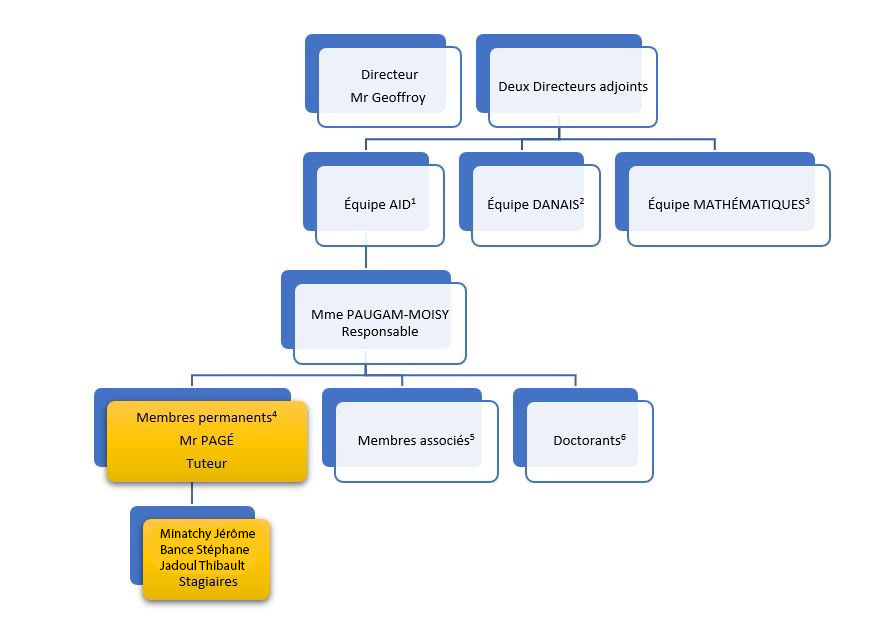
\includegraphics[width=10cm]{./images/orga.jpg}
%\caption{Figure 1 Schéma de l'organisation interne du LAMIA:
%¹Apprentissages Interactions Données. ²Data analytics and big data
%gathering with sensors. ³Mathématiques (analyse variationnelle, analyse
%numérique, EDP, analyse statistique, mathématiques discrètes). ⁴Membres
%permanents : Suzy Gaucher-Casalis~(MCF),~Enguerran
%Grandchamp~(MCF--HDR),~Jean-Luc Henry~(MCF),~Jimmy Nagau~(MCF),~Vincent
%Pagé(MCF),~Helene Paugam Moisy~(PR),~Sébastien Régis~(MCF),~Céline
%Rémi~(MCF).}
%\end{figure}

La prochaine section sera consacrée à la présentation de la thématique
de recherche du groupe SpikesTrain et de mon stage.

\hypertarget{Objectif_Spike}{%
\subsection{Le groupe Spiketrain}\label{Groupe_Spiketrain}}

Comme signalé plus haut, le groupe \textbf{Spikestrain} s'intéresse aux
techniques d'\textbf{Intelligence Artificielle}, plus spécifiquement à
l'\textbf{apprentissage automatique} dont l'objectif est de créer des
programmes capable d'apprendre à partir de bases d'exemples.

Actuellement, parmi les techniques permettant l'apprentissage
automatique, une se démarque et est très populaire : les
\textbf{réseaux de neurones artificiels}, notamment dans leur version
\emph{profonde} qui sont très utilisés par exemple par \textbf{Facebook™}
pour sa \textbf{reconnaissance faciale} ou encore par \textbf{Google™}
pour ses \textbf{robots} qui apprennent par \textbf{répétitions} à jouer
à des jeux de stratégies comme les échecs ou le Go.

Bien qu'un des axes de recherche du groupe \textbf{SpikeTrain} concerne les
neurones impulsionnels, ce ne sont pas ceux que nous avons utilisés dans ces
travaux, et ils ne seront pas évoqués dans ce rapport.


\hypertarget{Contexte}{%
\section{Contexte du stage}\label{Contexte}}

\hypertarget{Le-Challenge}{%
\subsection{Le Challenge: Classifier les Cachalots}\label{Le-Challenge}}

Le challenge "Dyni Odontocete Click Classification"
(https://challengedata.ens.fr/challenges/32) consiste à réaliser un classifieur qui classe des mammifères marins de dix espèces différentes à partir de leurs "clics", c'est à dire le son qu'ils émettent avec leur machoires.

Pour celà nous avions à disposition une \textbf{base labelisée} (comportant 113000 exemples) ainsi qu'une \textbf{base de test}, non labelisée (comportant 20000 exemples). Comme dans tout challenge de ce type, ces deux bases ont des rôles
très différents :

\begin{itemize}
  \item La \textbf{base labelisée} sera découpée en deux par les participants :
    \begin{itemize}
      \item une \textbf{base d'apprentissage} permettant de régler les
      paramètres des algorithmes.
      \item une \textbf{base de validation} permettant d'évaluer les
      performances des algorithmes sur des exemples qu'ils n'ont jamais vus.
    \end{itemize}
  \item La \textbf{base de test} sert pour l'évaluation par les organisateurs du
  challenge. Quotidiennement, les participants peuvent déposer leurs prédictions
  sur cette base (Deux fois par jour maximum). On peut ainsi définir les
  performances des différents participants.
\end{itemize}

Ci dessous, une traduction approximative du descriptif du challenge tel qu'il
est présenté sur le site dont j'ai donné l'adresse en tête de cette section :

\begin{quotation}
Les deux bases sont constituées d'enregistrements audios des clics des différentes espèces. Chaque enregistrement contient 8192 mesures faites à une fréquence d'échantillonnage de 200KHz. Dans le cas de la base non labelisée appellée base de test chaque enregistrement contient normalement un clic centré au milieu de la fenêtre tandis que dans la base labelisée appellée base d'apprentissage, le clic n'est pas spécialement centré et peut se situer à divers moments de l'enregistrement. De plus, les enregistrements peuvent contenir divers bruits.

L'objectif est de classer chaque enregistrement en fonction de l'espèce émettrice correspondante. Les 10 espèces sont :
\begin{itemize}
\item (0) Gg : Grampus griseus- Dauphin de Risso
\item (1) Gma : Globicephala macrorhynchus- Baleine pilote à nageoires courtes
\item (2) La : Lagenorhynchus acutus- Dauphin à flancs blancs de l'Atlantique
\item (3) Mb : Mesoplodon bidens- Baleine à bec de Sowerby
\item (4) Me : Mesoplodon europaeus- Baleine à bec de Gervais
\item (5) Pm : Physeter macrocephalus - Cachalot
\item (6) Ssp : Stenella sp.Dauphin stenellide
\item (7) UDA : Delphinidés de type A - un groupe de dauphins (espèces non encore déterminées)
\item (8) UDB : Delphinidés de type B - un autre groupe de dauphins (espèces non encore déterminées)
\item (9) Zc : Ziphius cavirostris - Baleine de Cuvier à bec.
\end{itemize}

La performance du classifieur est évaluée sur la base de test (les labels sont envoyés au site du challenge) par une mesure d'accuracy (le nombre de bien classés sur le nombre total d'exemples).
\end{quotation}

\hypertarget{Etat-des-lieux-lors-de-mon-arrivuxe9}{%
\subsection{Etat des lieux à mon arrivée}
\label{Etat-des-lieux-lors-de-mon-arrivuxe9}}

Quand j'ai commencé mon stage, mes tuteurs avaient déjà commencé le challenge depuis un moment déjà. J'ai ainsi dû, dans un premier temps, me mettre à jour
sur le challenge et ce qu'ils avaient fait, à savoir :

\begin{itemize}
\item Un grand nombre de tentatives de résolution du probléme uniquement basé sur du machine learning notament des réseaux de neurones et des réseaux de neurones convolutionnels
\item Divers traitements des signaux bruts
\item De l'augmentation de données
\end{itemize}

Leurs meilleurs résultats étaient les suivants :
\begin{itemize}
  \item de l'ordre de 98\% de réussite en accuracy sur la base de validation
  \item de l'ordre de 72\% de réussite sur la base de test
\end{itemize}

Cet un écart de 20 points entre les deux bases persistait même en utilisant
d'autres méthodes de machine learning donnant de moins bons résultats.
Cet important différentiel est d'autant plus surprenant que les auteurs du
challenge nous présentent les données de la base non labelisée comme des données
de meilleure qualité que celles de la base labelisée.

C'est pour mieux comprendre ce différentiel mais surtout le probléme dans son
ensemble que j'ai été chargé de créer un certain nombre d'outils facilitant
l'analyse et la visualisation des données et des effets des traitements que
nous leurs appliquons.

Avant de pouvoir commencer cette partie du travail, il m'a fallu prendre en main
un certain nombre de concepts et d'outils, concernant les \textbf{réseaux de neurones}, que nous allons voir ensemble maintenant.

\hypertarget{Neurone-artificiel}{%
\subsubsection{Neurone artificiel}
\label{Neurone-artificiel}}
Tout d'abord avant de parler de réseaux de neurones il faut expliquer le principe du neurone artificiel.

Un neurone artificiel est pourvu d'un certain nombre d'\textbf{entrées}. Dans le cas des neurones classiques, ces entrées sont des nombres réels. Le neurone calculera, en fonction de ces entrées, une unique valeur en \textbf{sortie}.
Détaillons la façon dont ces calculs sont effectués:

Chacune de ces entrées circule sur une connection, laquelle est caractérisée par un \textbf{poids} qui définit l'importance de l'entrée pour le neurone.

Le neurone calcule dans un premier temps la somme de ses entrées, pondérée par leurs poids respectifs, à laquel vient s'ajouter un \textbf{biais} spécifique à chaque neurone (cf. equation~\ref{sommePonderee}).

\begin{equation}
\label{sommePonderee}
y = \sum_{i}^{n} w_i \times x_i + b
\end{equation}

Le résultat de cette somme passe alors dans une \textbf{fonction d'activation} qui permet d'introduire une non-linéarité dans les calculs. La sortie $s$ du neurone est donc calculée conformément à l'équation~\ref{calcNeurone}

\begin{equation}
\label{calcNeurone}
s = f(\sum_{s=0}^{n_{x}} x_{n}w_{n} + b)
\end{equation}

Un schéma reprenant ces explications est présenté dans la figure~\ref{neuroneSeul}.

\begin{figure}[h]
\centering
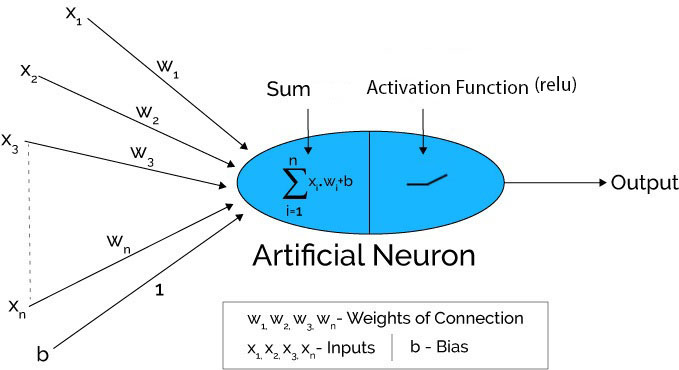
\includegraphics[width=10cm]{./images/image2.jpg}
\caption{Fonctionnement d'un neurone seul.\label{neuroneSeul}}
\end{figure}

Notre apprentissage se fera en modifiant les poids de ses différentes
connexions (et le biais) de façon à obtenir une sortie proche de celle voulue.

\hypertarget{Ruxe9seau-de-neurones-classique}{%
\subsection{Réseau de neurones classique}
\label{Ruxe9seau-de-neurones-classique}}

Les neurones présentés précédemment prennent tout leur intérêt lorsqu'ils sont utilisés en groupes, dans des \textbf{réseaux de neurones}.

Le premier de ces réseaux, encore utilisé de nos jours, est appelé \textbf{perceptron}.
Le principe du perceptron n'est pas nouveau et date des années 1960.

Dans ces types de réseaux, les neurones sont organisés en \textbf{couches} (une seul couche pour le perceptron et plusieurs pour le perceptron multicouche).
La première couche correspond à celle qui permettra d'introduire des informations dans le réseau (comme la rétine par exemple). Elle est nommée \textbf{couche d'entrée}
La dernière couche permettra de lire les décisions du réseau. Elle est appelée \textbf{couche de sortie}. Dans les applications classiques, à chaque neurone de la couche de sortie correspond une décision possible et le neurone qui est le plus activé sur la couche de sortie l'emporte.
Entre ces couches, on trouve souvent un nombre variable de couches intermédiaires appelées \textbf{couches cachées}.

Entre deux couches, on établit le plus souvent un schéma de connexion qualifiée
de \textit{full connected} ou \textit{dense}.
Dans ce cas, chaque neurone d'une couche est connecté avec chaque neurone de la
couche suivante. Pour le bien de ce rapport, nous n'épiloguerons pas sur les autres
types de connexions existantes. Ce type d'architecture est présentée sur la figure \ref{reseauClassique}.

\begin{figure}[h]
\centering
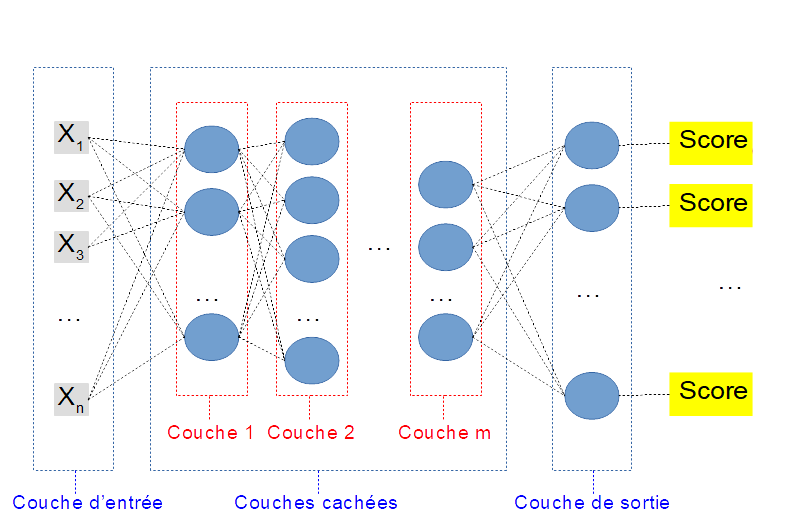
\includegraphics[width=10cm]{./images/multicouche.png}
\caption{réseau de neurones classique en couches.%
\label{reseauClassique}}
\end{figure}


\hypertarget{Ruxe9seau-de-neurones-convolutif}{%
\subsection{Réseau de neurones convolutifs}
\label{Ruxe9seau-de-neurones-convolutif}}

Les réseaux de neurones \textbf{convolutifs} sont un type de réseau de neurones
inspirés par le cortex cérébral des animaux.
Ils possèdent de larges applications dans la reconnaissance d'images, de vidéos
et de sons.

Ce réseau se présente comme un réseau classique , une couche d'entrée,
une couche de sortie et des couches cachées.
Ces couches cachées possèdent des couches \textbf{convolutives}
pour lesquelles chaque neurone va appliquer un filtre convolutif
sur une partie de l'image en entrée afin d'analyser toute l'image
(voir figure \ref{fig:explication_convolution}).

\begin{figure}[h!]
\centering
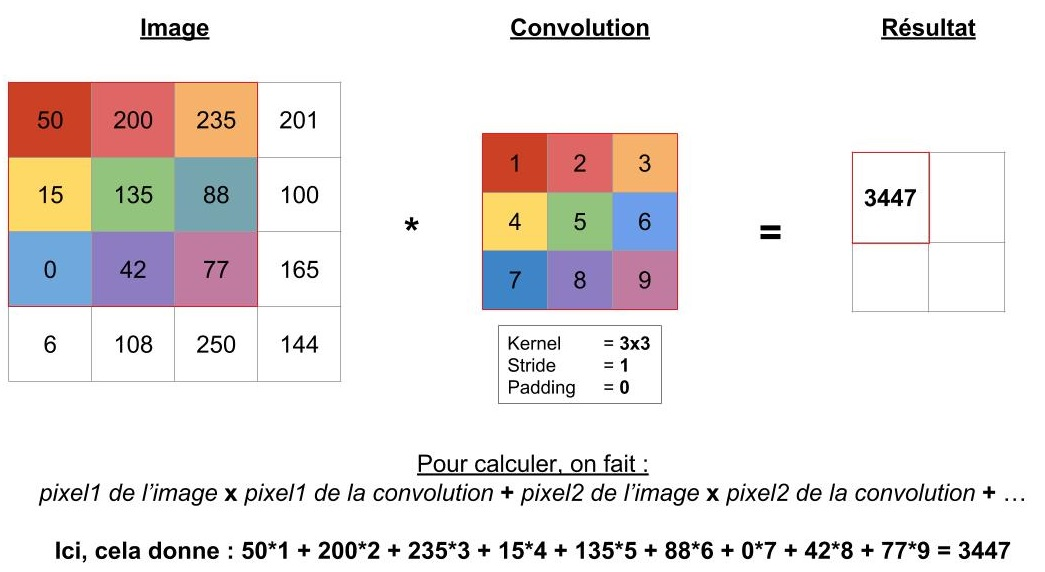
\includegraphics[width=12cm]{./images/explication_convolution.jpg}
\caption[Schéma de la convolution.]{L'image d'entrée est découpée en \textit{patchs}
sur lesquels est appliqué un filtre de convolution.
La sortie de ce fitre appliqué à chacun des patchs donne la couche de sortie
de la couche convolutive (appelée carte ou map).
La convolution est paramètrée par : le \textit{kernel} (la forme du patch),
le \textit{stride} (le déplacement du filtre) et le \textit{padding}
(la façon dont les bords de l'image vont être traités).
\label{fig:explication_convolution}}
\end{figure}

Dit autrement et pour simplifier, tous les neurones d'une couche travaillent
sur une portion de la couche précédente, limitée spatialement.
De plus, tous ces neurones partagent leur poids et effectuent dont la même
opération (de convolution) sur différentes parties des sorties de la couche
précédente.

Les réseaux convolutifs possèdent aussi des couches de \textbf{pooling}.
Le \textbf{pooling} est une opération simple qui consiste à remplacer une zone
de pixels (généralement 2×2 ou 3×3), par une valeur unique
(généralement le max ou la moyenne).
De cette manière, l’image diminue en taille et se retrouve simplifiée (lissée).

L'un des intérêts majeurs des réseaux convolutifs est qu'ils permettent de
réaliser une invariance de translation :
un motif appris sur une zone de l'image sera reconnue quelque soit sa position
dans l'image.
Un autre intérêt est qu'ils nécessitent l'apprentissage de beaucoup moins de
paramètres (les poids) que les réseaux de neurones de type Perceptron
Multicouche, pour des performances en classification équivalentes ou
supérieures.

\hypertarget{plan}{%
\section{Présentation du plan du rapport}%
\label{Présentation du plan du rapport}}

Ceci ayant été posé, nous pouvons maintenant présenter le plan de ce rapport,
qui sera structuré comme suit :

Après ce chapitre d'introdution, qui présentait le contexte opérationnel, la mission et les pré-requis théoriques de ce stage, le
chapitre~\ref{Analyse-et-traitement-des-donnuxe9es} présentera l'essentiel
des travaux que j'ai réalisés durant ce stage.

Mon objectif était de permettre au groupe spike de visualiser les signaux
injectés dans les réseaux de neurones.
Les signaux issus des bases d'exemples du challenge seront présentés dans la section~\ref{Les-signaux}.
Ces signaux passent ensuite au travers d'une multitude de filtres.
Certains de ces filtres ont un objectif de prétraitement et seront vus en section~\ref{Traitement-du-signal}).
D'autres filtres sont là pour faire de l'\textbf{augmentation de données}, ce
qui occupera la section~\ref{Data-augmentation} que nous avons laissée sous son
nom anglophone (\textit{Data Augmentation}) comme c'est le cas dans toutes les documentations que nous avons
trouvées.
Pour organiser le passage des signaux des bases d'exemples vers l'entrée des réseaux de neurones, les framework actuel de réseaux de neurones utilisent
la notion de \textbf{pipeline de données}, que mes tuteurs et moi même avons
fouillés au cours de ce stage. Ils font l'objet de la
section~\ref{Les-Pipelines}.
Enfin, l'objectif final de mes travaux était de produire des outils permettant
de générer rapidement des fiches synthétisant les visualisations des signaux à divers emplacement de ce pipeline. Ces fiches et les outils permettant de les
créer sont décrits dans la section~\ref{Les-PDF}.

Cette année 2020 a été très particulière en raison du confinement lié au
COVID-19. Ce stage ayant, comme l'ensemble des activités mondiales, a été
impacté par ce confinement et a été réalisé en intégralité sous forme de
travail à distance. Il nous a semblé judicieux d'ajouter à ce rapport un
chapitre dédié à ces spécificités (cf. chapitre~\ref{Le-travail-a-distance}).

Enfin, nous terminerons ce rapport par une conclusion et des perspectives.
